\chapter{Analysis}


\section{State of the art}
	\subsection{Noteput}
		German table where you physically put notes on it, and press play button to play notes, hopefully learning note and sheet theory.
	\subsection{Dato duo}
		Two person synthesizer for kids, to play around with, no apparent learning outcome, but seems fun to play around with.
		\begin{figure}[H]
			\centering
			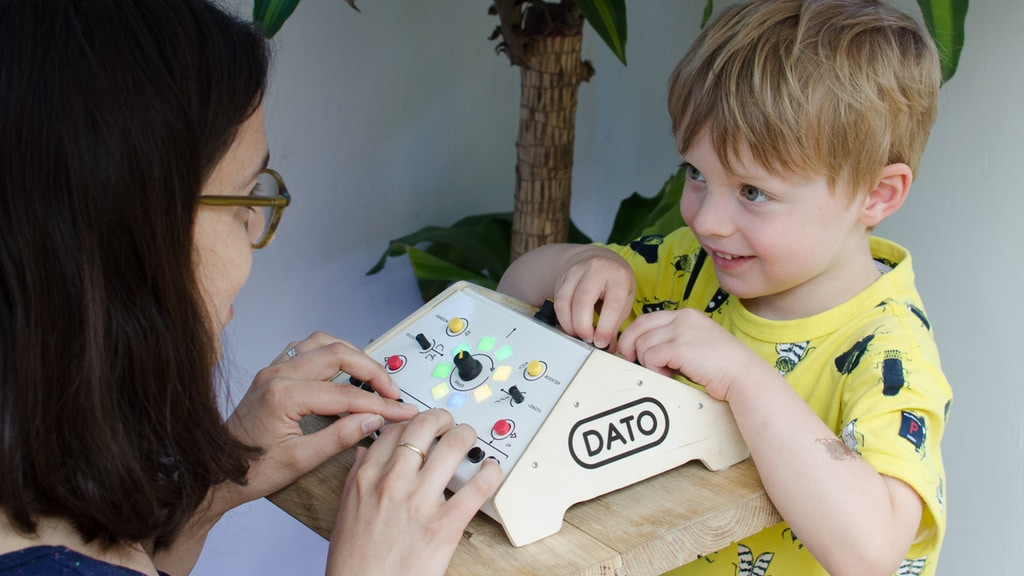
\includegraphics[width=0.7\linewidth]{figure/Analysis/datoduo}
			\label{fig:datoduo}
			\caption{Dato duo synthesizer}
		\end{figure}
	\subsection{Soundstage}
		VR application by Google, where you compose and play music in virtual reality. You can synthesize, plug things into other things, and create entire scores in this virtual reality playground.
		
	\subsection{V-Beat}
		The v-beat drumsticks are, for all its intents and purposes, simply air drumming.
		\begin{figure}[H]
			\centering
			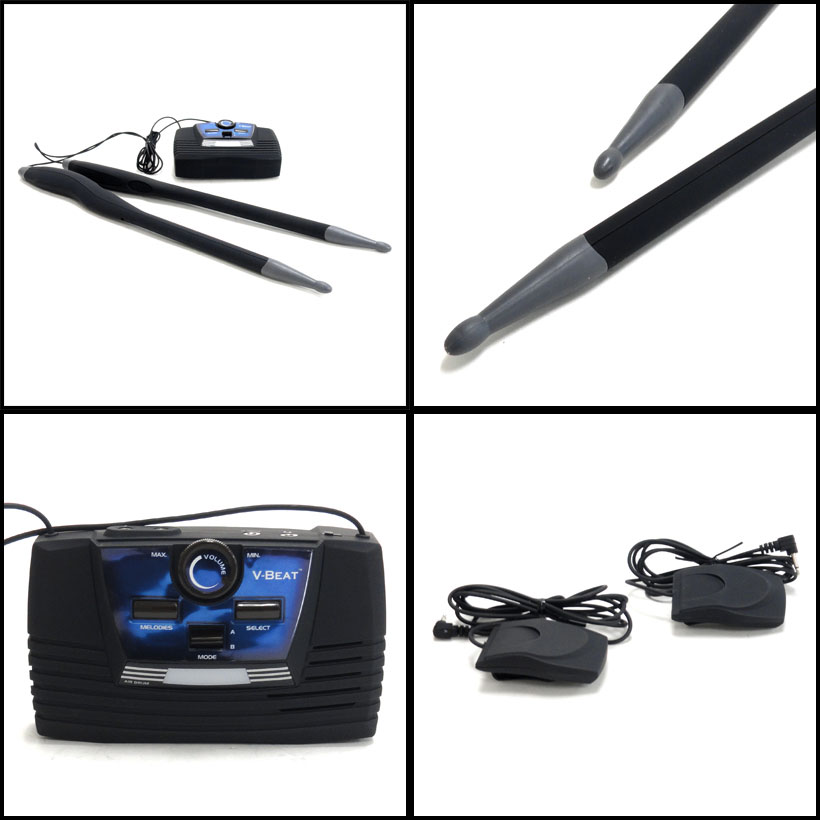
\includegraphics[width=0.5\linewidth]{figure/Analysis/vbeat}
			\label{fig:vbeat}
			\caption{Vbeat drumsticks}
		\end{figure}
		
	\subsection{MI Guitar}
		\begin{figure}[H]
			\centering
			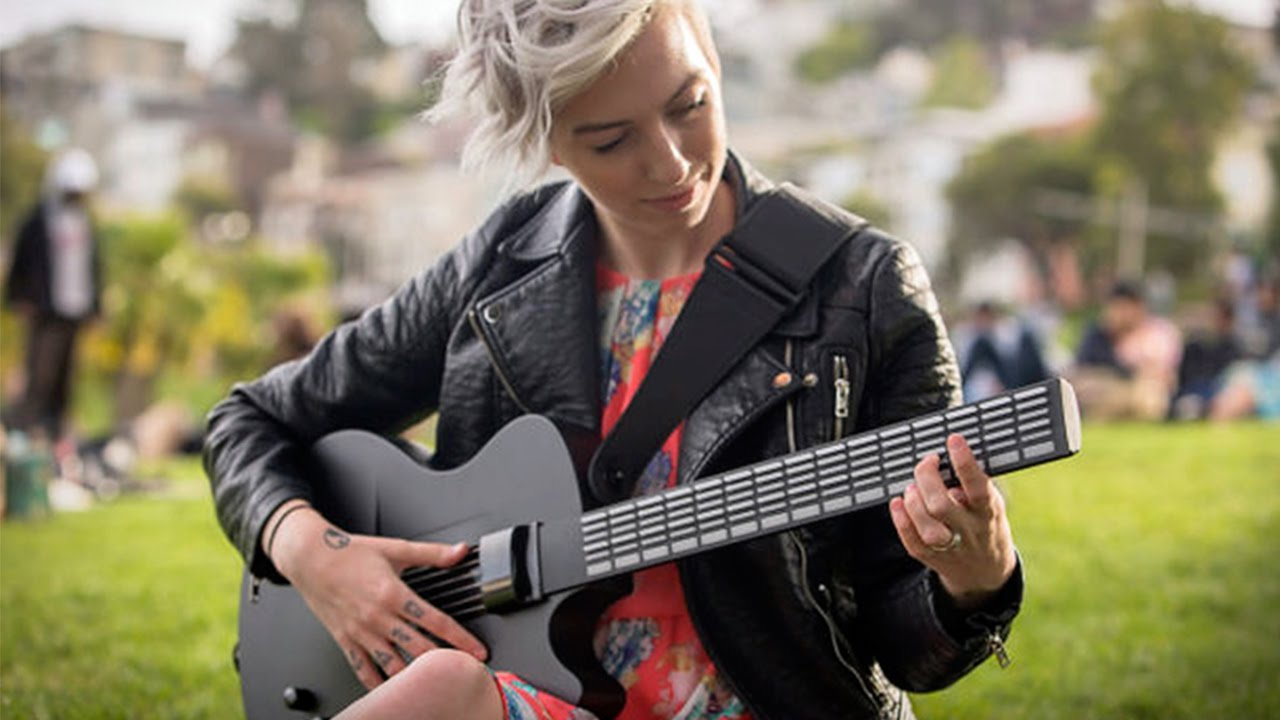
\includegraphics[width=0.8\linewidth]{figure/Analysis/miguitar}
			\label{fig:miguitar}
			\caption{MI guitar to teach guitar play}
		\end{figure}
	
	\subsection{Yousician}
		\begin{figure}[H]
			\centering
			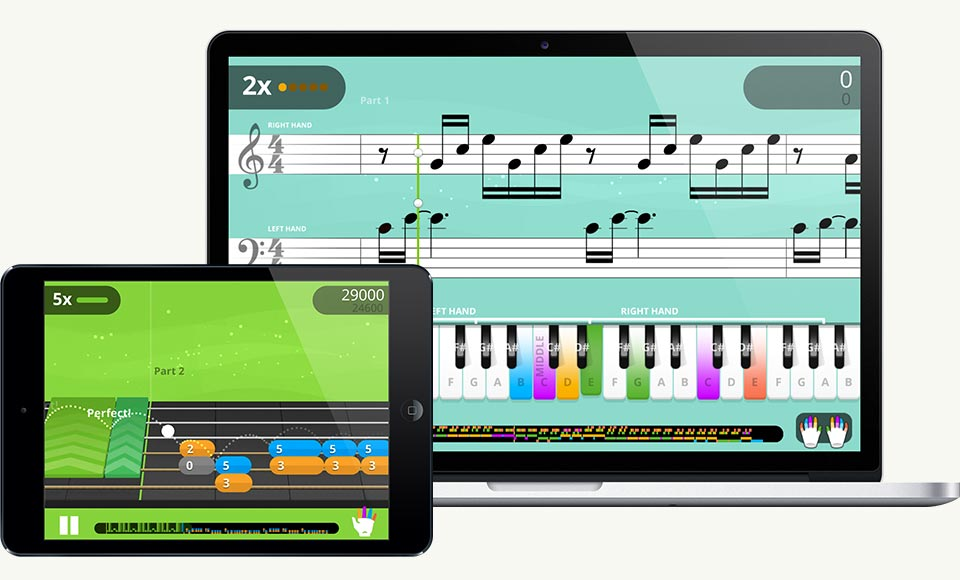
\includegraphics[width=0.8\linewidth]{figure/Analysis/yousician.jpg}
			\label{fig:yousician}
			\caption{Yousician}
		\end{figure}
	
	\subsection{Chrome Music Lab}
		\begin{figure}[H]
			\centering
			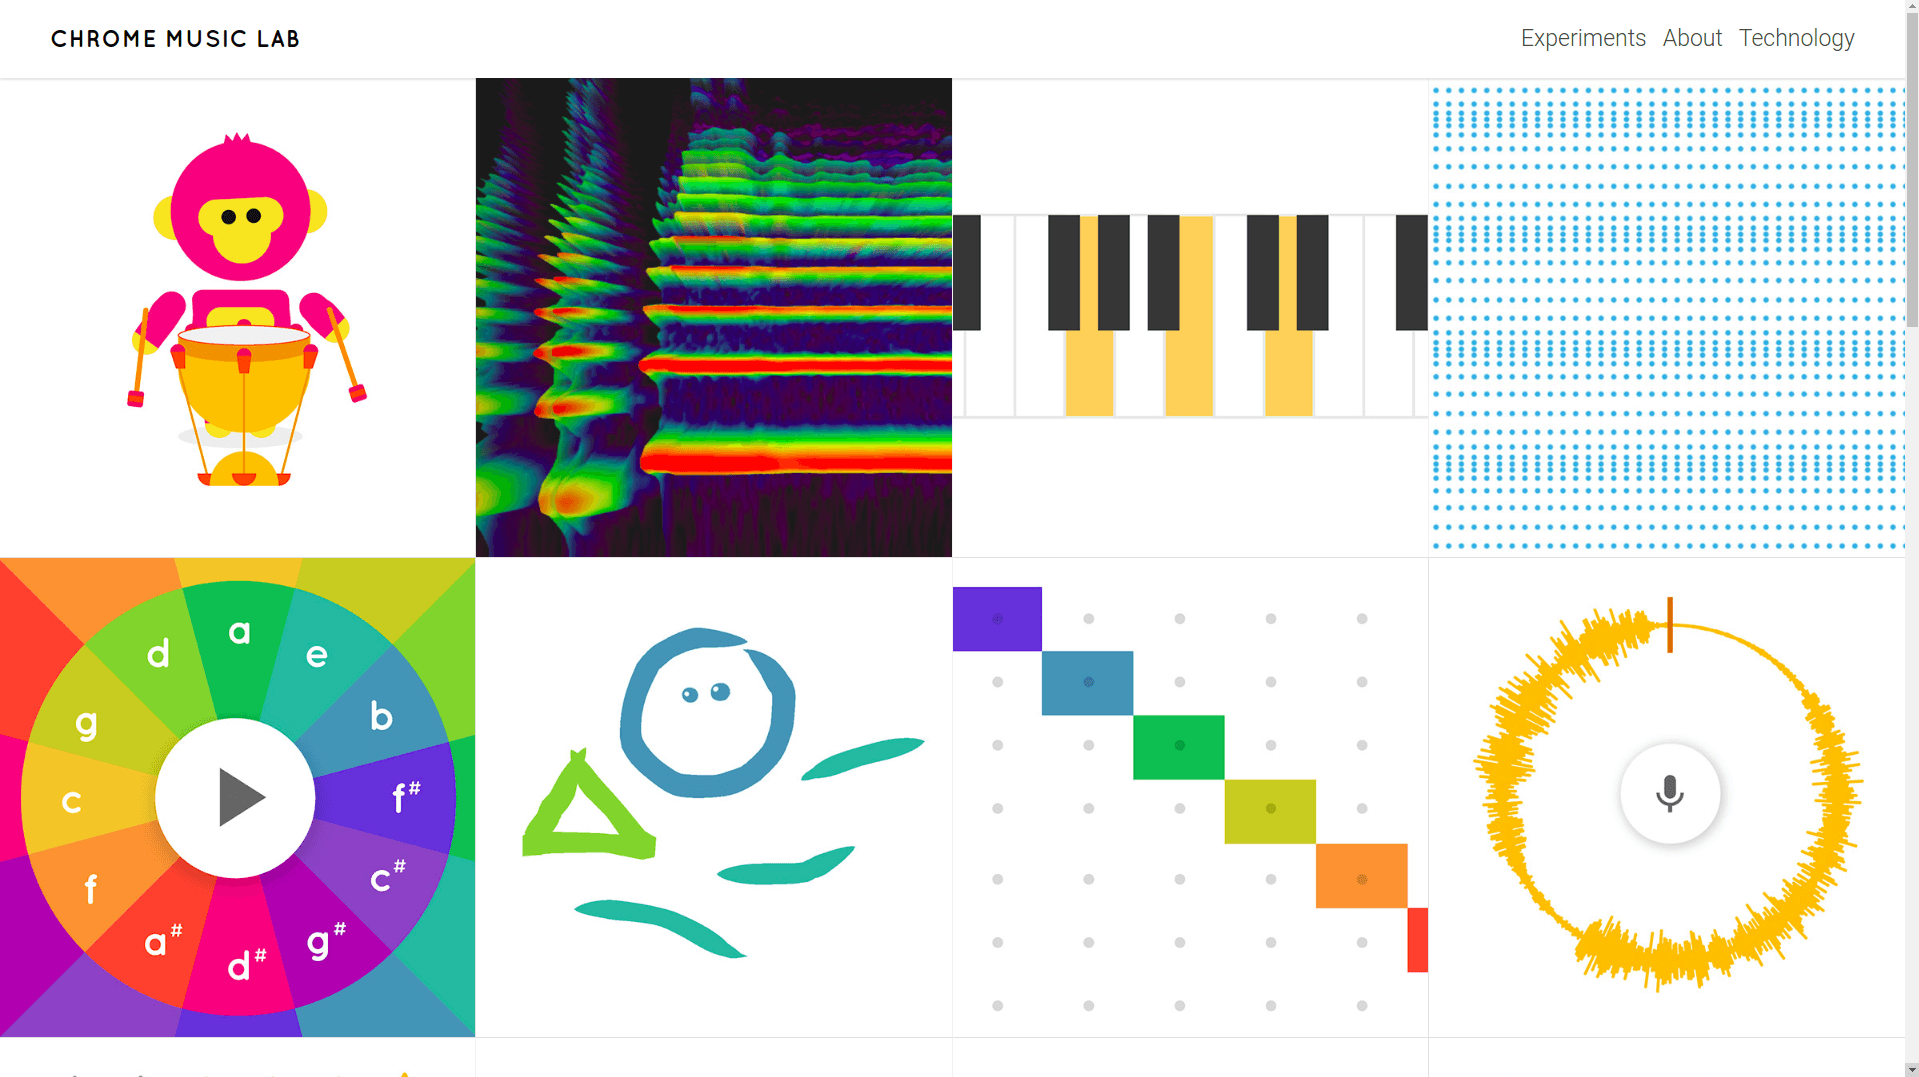
\includegraphics[width=0.8\linewidth]{figure/Analysis/chromeMusicLab.png}
			\label{fig:chromeMusicLab}
			\caption{Chrome Music Lab}
		\end{figure}

		